\documentclass[final,t]{beamer}
\usepackage[size=a0,scale=1.50,orientation=portrait]{beamerposter}
\usetheme{default}
\setbeamertemplate{navigation symbols}{}
\setbeamertemplate{headline}{}
\setbeamertemplate{footline}{}
\setbeamersize{text margin left=6mm, text margin right=6mm}
\setbeamertemplate{blocks}[rounded][shadow=false]

\usepackage{helvet}
\renewcommand{\familydefault}{\sfdefault}
\usepackage[utf8]{inputenc}
\usepackage{graphicx}
\usepackage{booktabs}
\usepackage{hyperref}
\hypersetup{colorlinks=true,urlcolor=blue}

\definecolor{utpblue}{RGB}{8,55,106}
\definecolor{utpred}{RGB}{168,19,32}
\definecolor{softgray}{RGB}{243,246,250}
\definecolor{textgray}{RGB}{28,32,36}

\setbeamercolor{normal text}{fg=textgray,bg=white}
\setbeamercolor{structure}{fg=utpblue}
\setbeamercolor{block title}{fg=white,bg=utpblue}
\setbeamercolor{block body}{fg=textgray,bg=softgray}
\setbeamercolor{block title alerted}{fg=white,bg=utpred}
\setbeamercolor{block body alerted}{fg=textgray,bg=softgray}

\setbeamerfont{title}{size=\LARGE,series=\bfseries}
\setbeamerfont{author}{size=\Large,series=\mdseries}
\setbeamerfont{institute}{size=\normalsize}
\setbeamerfont{block title}{size=\large,series=\bfseries}
\setbeamerfont{block body}{size=\large}

\setlength{\columnsep}{0.7cm}
\setlength{\leftmargini}{1.1em}
\setlength{\itemsep}{0.16cm}
\linespread{1.05}
\emergencystretch=1.8em

\title{Conformal Prediction para Calibración e Incertidumbre en Riesgo Crediticio}
\author{Carlos Alfredo Vergara Rojas}
\institute{Tesis de Especialización en Analítica y Ciencia de Datos Aplicada}

\begin{document}
\begin{frame}[t]

\begin{beamercolorbox}[wd=\linewidth,sep=0.42cm,leftskip=0.6cm,rightskip=0.6cm,rounded=true]{block title}
  \begin{columns}[T,totalwidth=\linewidth]
    \begin{column}{0.84\linewidth}
      \centering
      {\usebeamerfont{title}\inserttitle}\\[0.12cm]
      {\large Aplicación en Lending Club para PD/LGD/EAD e impacto IFRS9}\\[0.12cm]
      {\usebeamerfont{author}\insertauthor}\\[0.08cm]
      {\usebeamerfont{institute}\insertinstitute}
    \end{column}
    \begin{column}{0.14\linewidth}
      \centering
      
\includegraphics[width=0.72\linewidth]{figures/logo-utp.jpg}
    \end{column}
  \end{columns}
\end{beamercolorbox}

\vspace{0.30cm}

\begin{columns}[t,totalwidth=\linewidth]

\begin{column}{0.325\linewidth}

  \begin{block}{Problema, objetivo y aporte de la tesis}
    \begin{itemize}
      \item En riesgo crediticio, una predicción puntual sirve para ranking, pero no para decidir con prudencia provisión, capital o pricing.
      \item Objetivo central: pasar de ``modelo que predice'' a \textbf{modelo defendible para decidir bajo incertidumbre}.
      \item Aporte: integrar calibración y predicción conformal en PD/LGD/EAD con evidencia trazable en un caso real (Lending Club).
    \end{itemize}
  \end{block}

  \vspace{0.26cm}

  \begin{block}{Datos y estructura del riesgo (OOT)}
    \begin{itemize}
      \item Train: 1,346,311 (18.52\% default)
      \item Calibration: 237,584 (22.20\%)
      \item Test: 276,869 (21.98\%)
    \end{itemize}
    \vspace{0.15cm}
    \begin{center}
      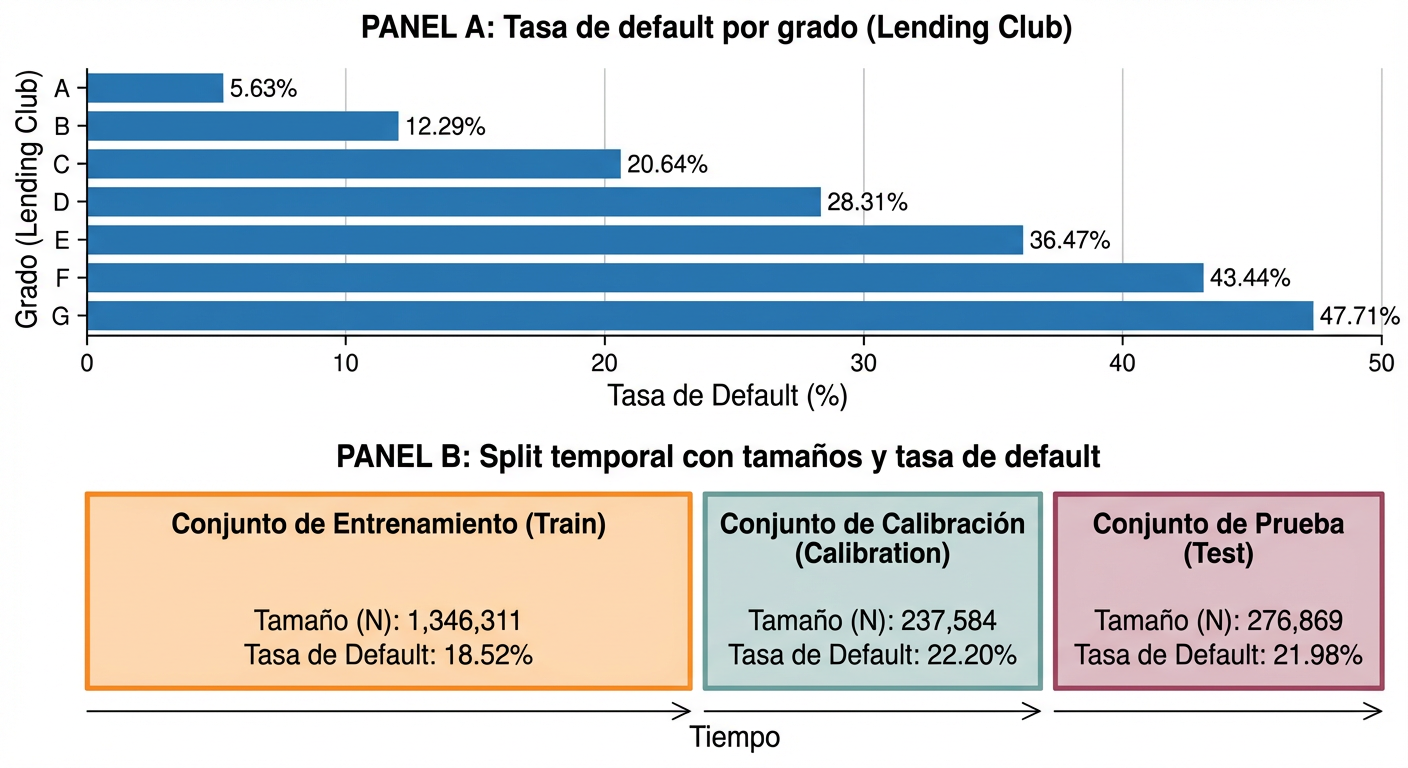
\includegraphics[width=0.98\linewidth]{figures/figure1.png}
    \end{center}
  \end{block}

\end{column}

\begin{column}{0.335\linewidth}

  \begin{block}{Resultados PD y calibración}
    \begin{columns}[T,totalwidth=\linewidth]
      \begin{column}{0.48\linewidth}
        \small
        \textbf{PD OOT}\\
        AUC: 0.7117\\
        Gini: 0.4234\\
        Brier: 0.1548\\
        ECE: 0.0072\\[0.18cm]
        \textbf{Cobertura conformal}\\
        90\% objetivo: 91.67\%\\
        95\% objetivo: 95.59\%
      \end{column}
      \begin{column}{0.50\linewidth}
        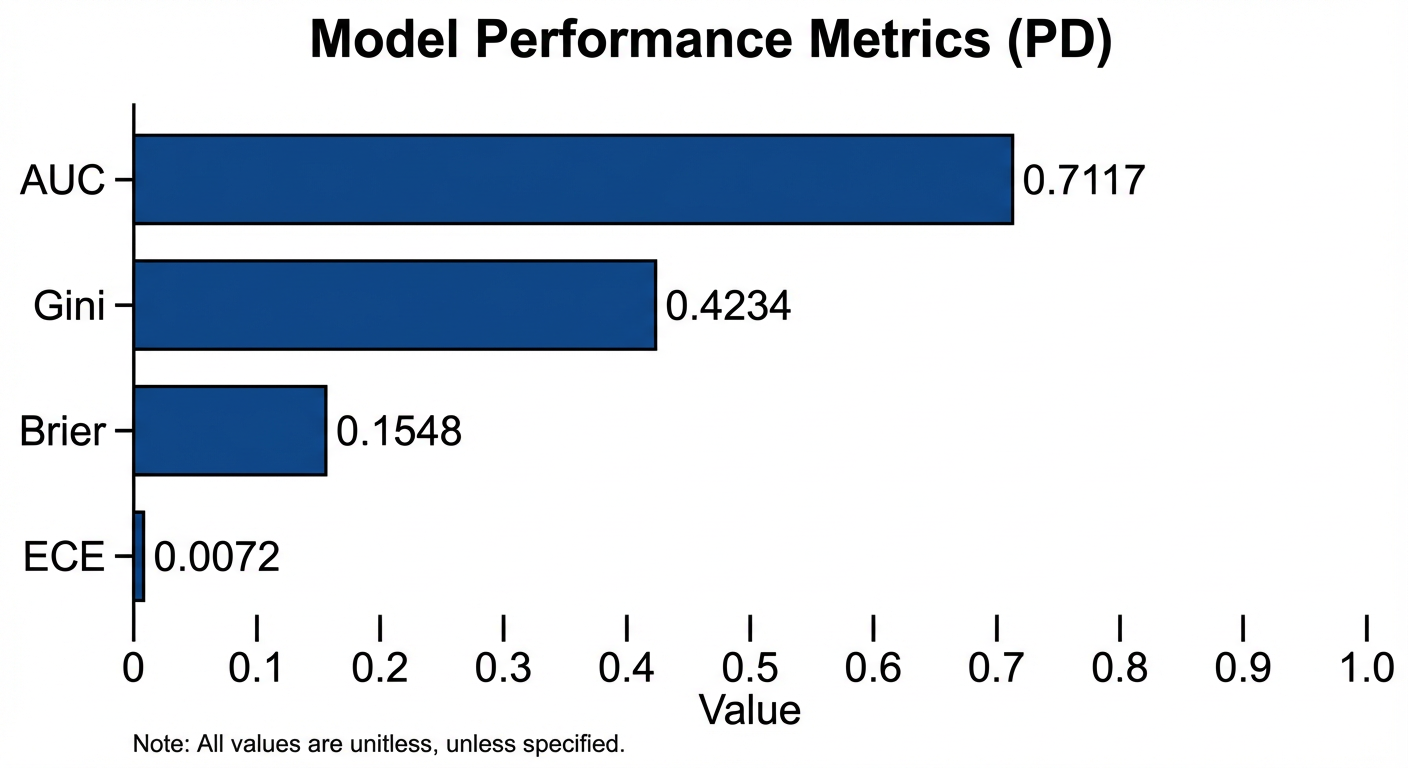
\includegraphics[width=\linewidth]{figures/figure2.png}
      \end{column}
    \end{columns}
  \end{block}

  \vspace{0.26cm}

  \begin{block}{Resultados LGD/EAD en la corrida actual}
    \small
    \textbf{LGD (variante seleccionada: direct\_adaptive\_grade\_temporal)}\\
    Coverage 90\%: 90.50\% \quad Coverage 95\%: 95.50\%\\
    Width 90\%: 0.4959 \quad Width 95\%: 0.5744\\[0.14cm]
    \textbf{EAD}\\
    Coverage 90\%: 91.37\% \quad Coverage 95\%: 95.45\%\\
    Width 90\%: 160.88 \quad Width 95\%: 241.88\\[0.14cm]
    \textbf{Lectura:} la brecha principal ya no es disponibilidad, sino sostener estabilidad de cobertura y eficiencia en monitoreo.
  \end{block}

  \vspace{0.26cm}

  \begin{block}{Evidencia conformal por grado}
    \begin{center}
      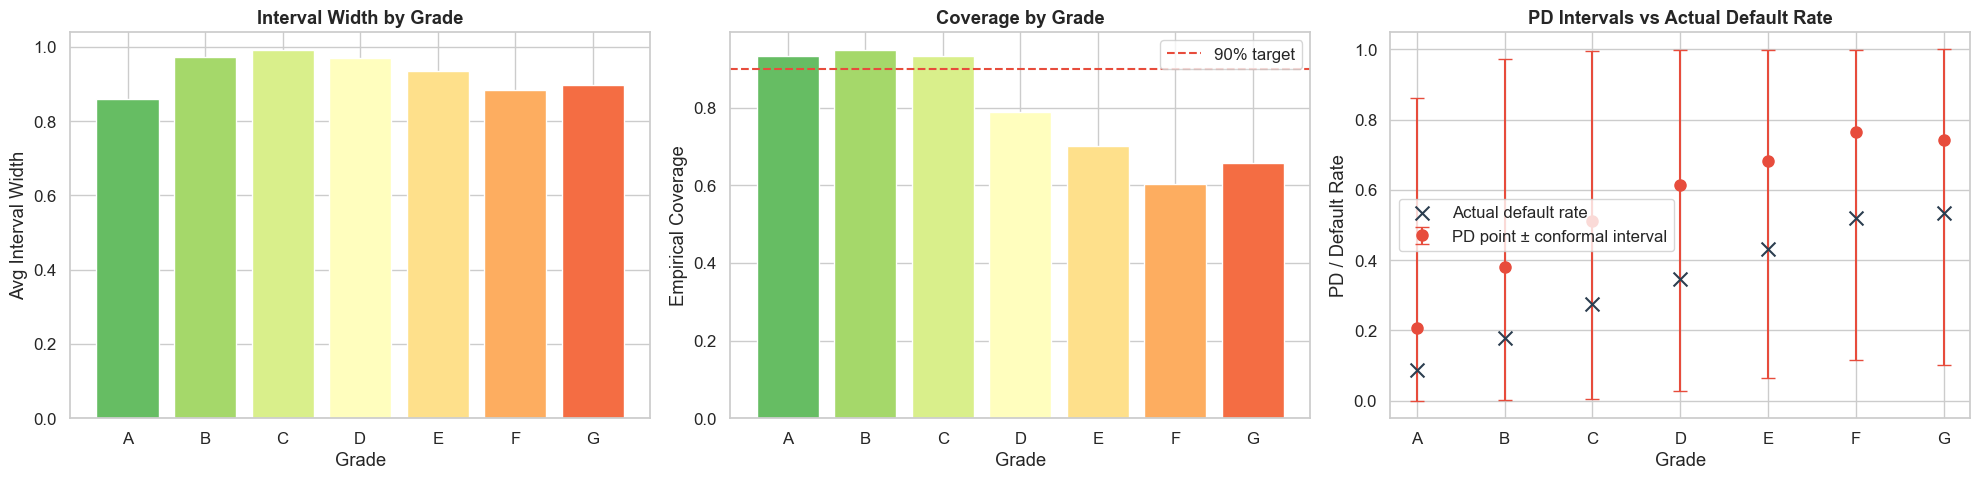
\includegraphics[width=\linewidth]{../reports/notebook_images/04_conformal_prediction/cell_012_out_01.png}
    \end{center}
    \vspace{-0.18cm}
    \small La cobertura por segmento permite diagnóstico granular y control técnico de riesgo por bucket.
  \end{block}

\end{column}

\begin{column}{0.325\linewidth}

  \begin{alertblock}{Impacto IFRS9 (ECL por escenario)}
    \begin{itemize}
      \item Baseline: 976.7M USD
      \item Mild stress: 1,200.0M USD
      \item Adverse: 1,463.0M USD
      \item Severe: 1,791.0M USD
    \end{itemize}
    \vspace{0.04cm}
    \begin{center}
      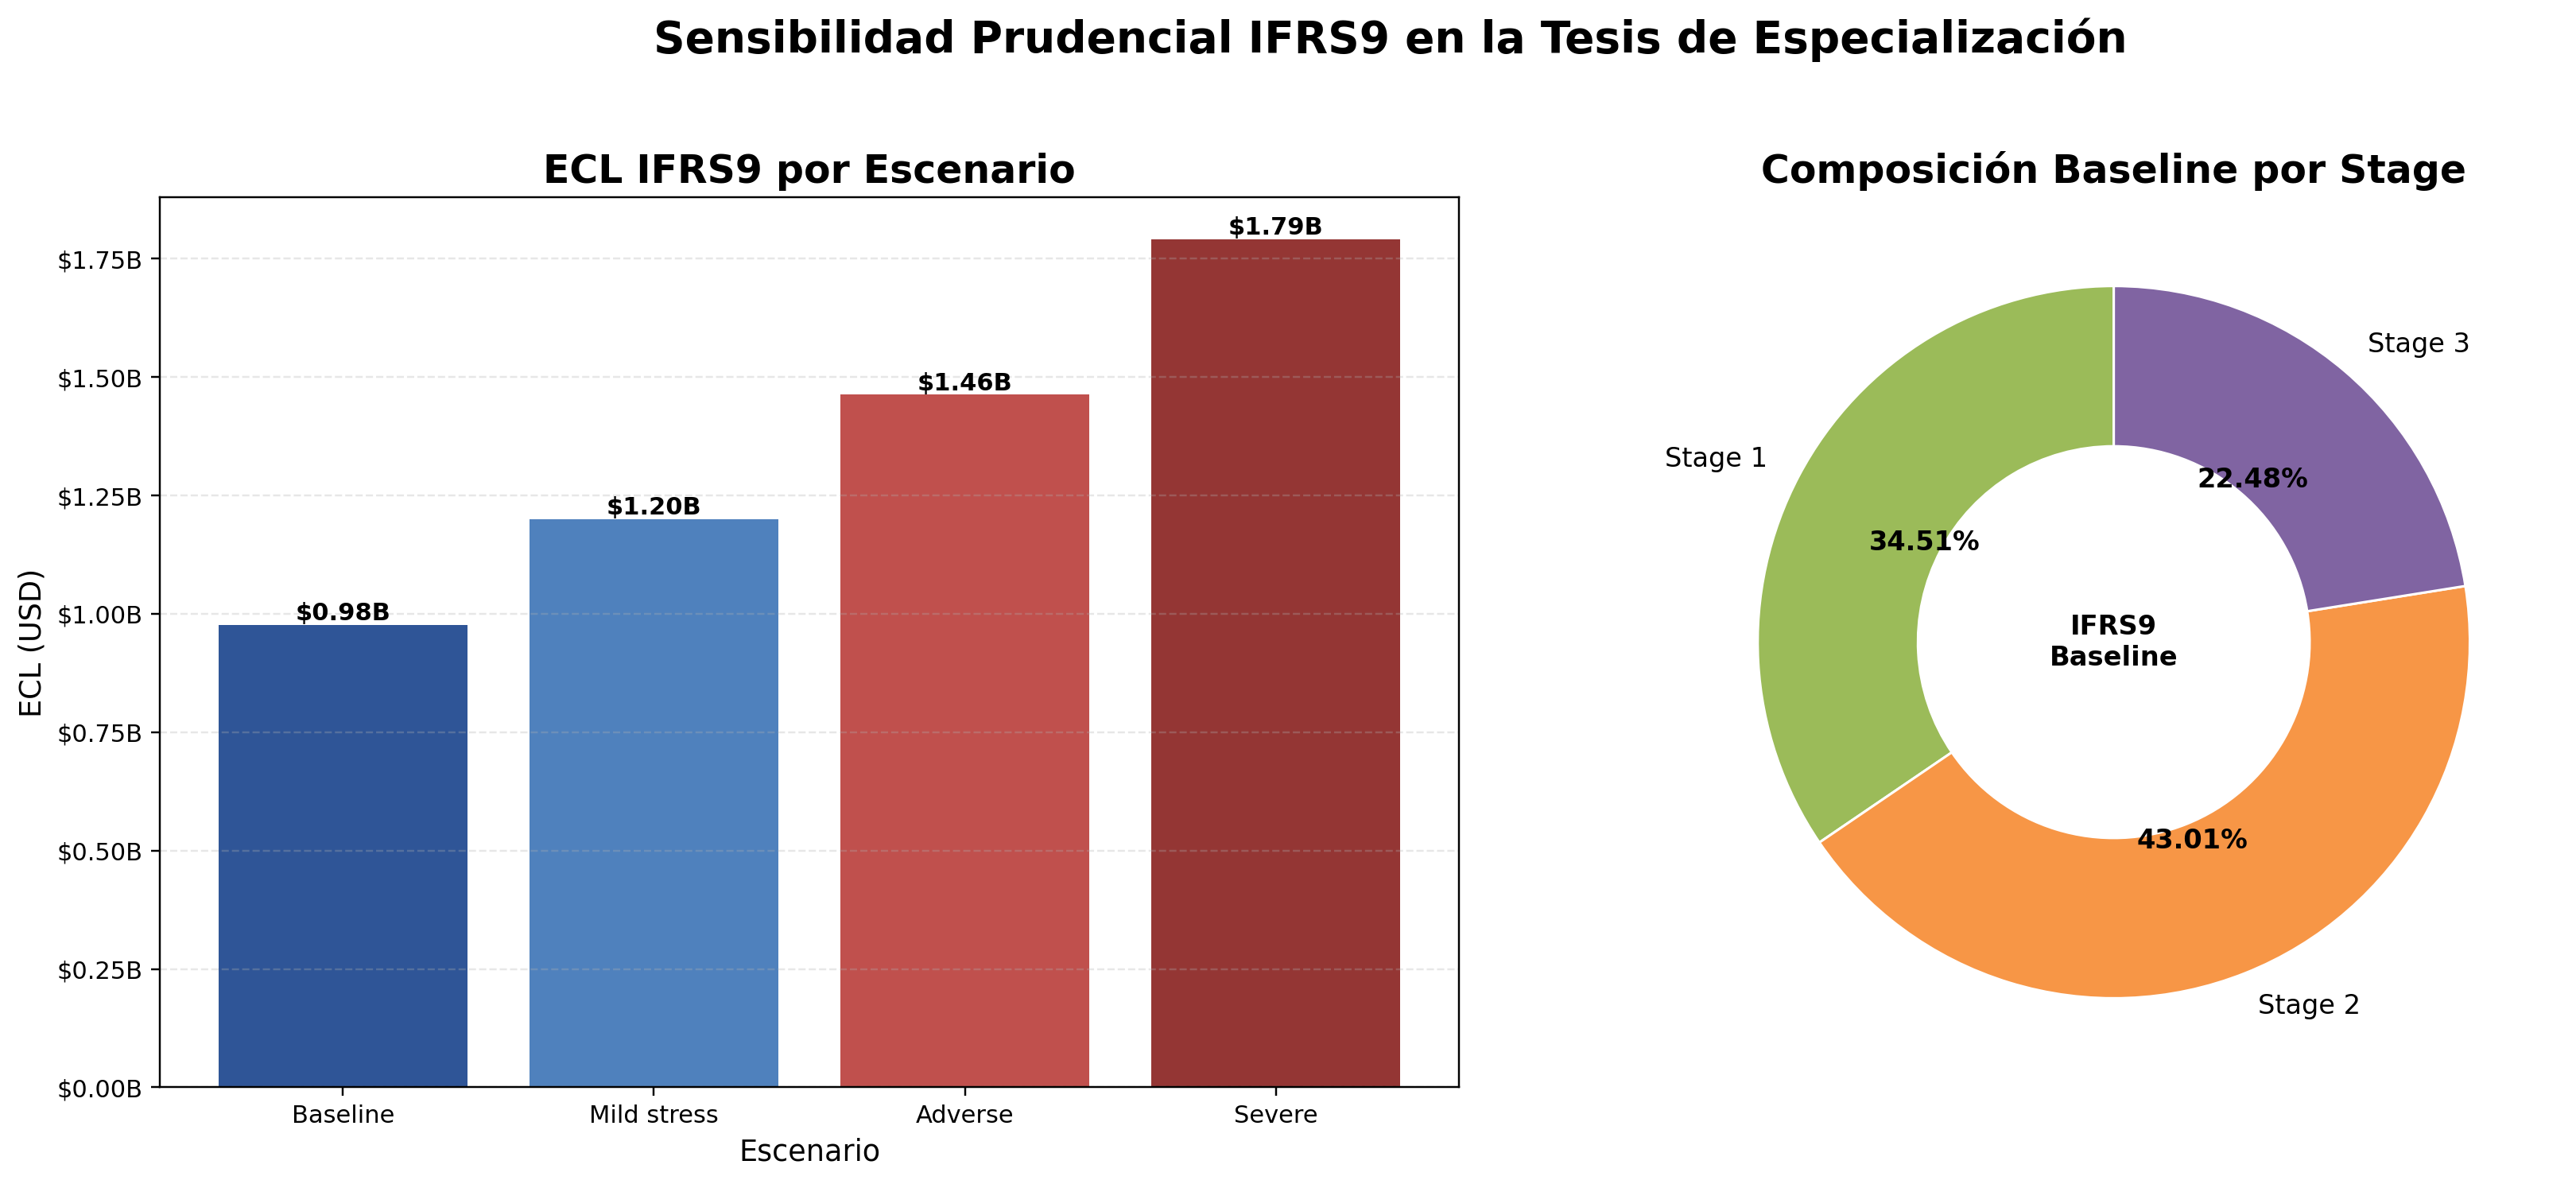
\includegraphics[width=\linewidth]{figures/figure3.png}
    \end{center}
  \end{alertblock}

  \vspace{0.26cm}

  \begin{block}{Conclusiones}
    \begin{itemize}
      \item La tesis integra contexto, teoría, datos, metodología y resultados con evidencia ejecutable.
      \item PD queda consolidado con calibración defendible para decisión.
      \item LGD y EAD muestran evidencia conformal en la corrida canónica.
      \item IFRS9 se conecta a escenarios y stages con lectura técnica y de negocio.
      \item El valor práctico es reducir sobreconfianza y mejorar defendibilidad regulatoria.
    \end{itemize}
  \end{block}

\end{column}
\end{columns}

\vspace{0.22cm}

\begin{block}{Próximos trabajos}
  \begin{columns}[T,totalwidth=\linewidth]
    \begin{column}{0.45\linewidth}
      \vspace*{0.50cm}
      \normalsize
      \begin{itemize}
        \item Integrar intervalos conformales en un modelo de optimización de portafolio para decisiones más robustas de capital, provisión y rentabilidad.
        \item Incorporar análisis de supervivencia para modelar el \textit{timing} de eventos de riesgo y enriquecer la lectura temporal del crédito.
        \item Agregar \textit{causal machine learning} para estimar efectos de políticas de originación/pricing y soportar decisiones de intervención.
        \item Integrar un pipeline end-to-end unificado (datos, modelado, evaluación, IFRS9 y monitoreo) para operación continua y trazable.
      \end{itemize}
    \end{column}
    \begin{column}{0.53\linewidth}
      \begin{center}
        \includegraphics[width=\linewidth]{figures/methods_flowchart_v1.png}
      \end{center}
    \end{column}
  \end{columns}
\end{block}

\end{frame}
\end{document}
